\chapter{第一次作业}\label{chap:hw1}

本次作业练习排序和图搜索。代码用 \lstinline|lstlisting| 排版，伪代码用
\texttt{algorithmic}，手写部分是扫描的 PDF。

\section{插入排序}\label{sec:insertion}

\subsection{代码}

下面的函数原地排序，调用方式是 \lstinline{insertion_sort(xs)}：
\begin{lstlisting}[language=Python,caption={插入排序 Insertion sort}]
def insertion_sort(xs):
    """Sort xs in place."""
    # In-place sort.
    for i in range(1, len(xs)):
        key, j = xs[i], i - 1
        while j >= 0 and xs[j] > key:   # 比 key 大的右移
            xs[j + 1] = xs[j]
            j -= 1
        xs[j + 1] = key
\end{lstlisting}

\subsection{复杂度}

最坏情况比较 $\frac{n(n-1)}{2}$ 次，所以时间是 $O(n^2)$。

\begin{enumerate}
  \item 最好情况：输入已经有序，只比较 $n-1$ 次；
  \item 平均情况：仍然是 $\Theta(n^2)$。
\end{enumerate}

\section{广度优先搜索}\label{sec:bfs}

\begin{algorithm}
  \caption{广度优先搜索 BFS}\label{alg:bfs}
  \begin{algorithmic}[1]
    \Procedure{BFS}{$G, s$}
      \State $Q \gets [s]$, 标记 $s$
      \While{$Q$ 非空}
        \State $u \gets$ \Call{Pop}{$Q$}
        \For{$v \in \mathrm{Adj}(u)$}
          \If{$v$ 未标记} \State 标记 $v$，\Call{Push}{$Q, v$} \EndIf
        \EndFor
      \EndWhile
    \EndProcedure
  \end{algorithmic}
\end{algorithm}

算法~\ref{alg:bfs} 每个顶点进出队列各一次，总时间 $O(|V| + |E|)$。

\section{手写部分}\label{sec:scan}

第 3 题的推导是手写的，扫描件附在下一页。

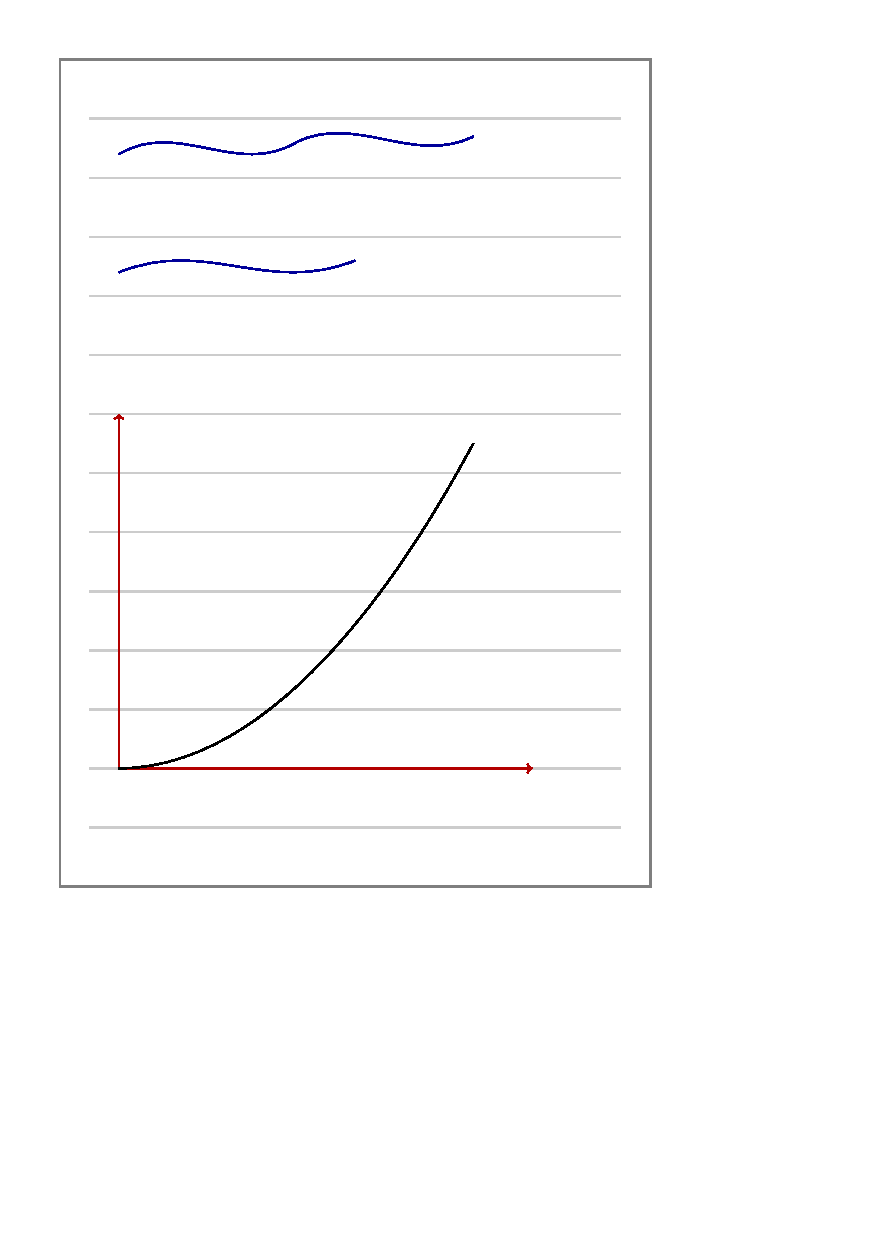
\includepdf[pages=1]{figures/scan.pdf}
